%% ===============================================
%% =============== Document Class ================
%% ===============================================



\documentclass[12pt,a4paper,openright]{book}



%% ===============================================
%% =============== Packages ======================
%% ===============================================



%% Language Support
\usepackage[T1,T2A] 		{fontenc}
\usepackage[utf8]   		{inputenc}
\usepackage[english,russian]{babel}
\usepackage{microtype}

%% Math

\usepackage{amsmath}
\usepackage{amsthm}
\usepackage{amssymb}
\usepackage{mathtext}

%% Layout
%\usepackage{a4wide}
\usepackage{lipsum}
\usepackage{newfloat}
\usepackage{caption}
\usepackage{titlesec}
\usepackage{fancybox, fancyhdr} %% Colontitles
\usepackage{indentfirst}
\usepackage{geometry}
\usepackage{hyperref}
\usepackage{mdframed}
\usepackage{graphicx}
\usepackage{subfig}
\usepackage{enumitem}
\usepackage[titletoc,toc]{appendix}
\usepackage{csquotes}
\usepackage{algorithm2e}

%% Syntax highlighting
\usepackage[cache=false,newfloat]{minted}
\usemintedstyle{vs}



\DeclareGraphicsExtensions{.pdf,.png,.jpg}
\graphicspath{{./img/}}

\theoremstyle{definition}
\newtheorem{definition}{\textls[150]{Определение}}[chapter]

\theoremstyle{definition}
\newtheorem{problem}{\textls[150]{Задача}}[chapter]

\setlist{nosep}



\usepackage{caption}
%%\usepackage{subcaption}
\captionsetup[listing]{name=Листинг,justification=centering}
\captionsetup[figure]{justification=centering}



%% ===============================================
%% =============== Layout ========================
%% ===============================================



\geometry{left=1cm}
\geometry{right=2cm}
\geometry{top=2cm}
\geometry{bottom=2cm}


%%\SetupFloatingEnvironment{listing}{name=Листинг}



\numberwithin{equation}{chapter}



\makeatletter

\titleformat
{\chapter} % command
[display] % shape
{\bfseries\huge} % format
{\slshape\MakeUppercase{\ifnum\pdfstrcmp{\@currenvir}{appendices}=0\appendixname\else\chaptername\fi} \thechapter} % label
{0.5ex} % sep
{
	\rule{\textwidth}{1pt}
	\vspace{1ex}
	\centering
} % before-code
[
\vspace{-0.5ex}%
\rule{\textwidth}{0.3pt}
] % after-code

\titleformat
{\section} % command
[block] % shape
{\bfseries\Large} % format
{\S\ \thesection\quad} % label
{0.5ex} % sep
{} % before-code
[] % after-code

\makeatother



%% Headers and footers
\pagestyle{fancy}
\fancyhf{}
\fancyhead[LE]{\slshape\leftmark}
\fancyhead[RE]{$\blacksquare$\ \bfseries\thepage}
\fancyhead[RO]{\slshape\rightmark}
\fancyhead[LO]{\bfseries\thepage\ $\blacksquare$}
\renewcommand{\headrulewidth}{1px}
\fancyfoot[LE]{\slshape\rightmark}
\fancyfoot[RE]{$\blacksquare$\ \bfseries\thepage}
\fancyfoot[RO]{\slshape\leftmark}
\fancyfoot[LO]{\bfseries\thepage\ $\blacksquare$}
\renewcommand{\footrulewidth}{1px}



\renewcommand{\cleardoublepage}{\clearpage}



\makeatletter
\renewcommand{\@biblabel}[1]{#1.}
\makeatother



\makeatletter
\let\ps@plain\ps@empty
\makeatother



\hypersetup{
	colorlinks,
	citecolor=black,
	filecolor=black,
	linkcolor=black,
	urlcolor=black
}
\renewcommand{\sectionautorefname}{\S}
\newcommand{\definitionautorefname}{опр.}

\makeatletter
\renewenvironment{minted@colorbg}[1]{
    %\setlength{\fboxsep}{-\fboxrule}
    \def\minted@bgcol{#1}
    \noindent%
    \begin{lrbox}{\minted@bgbox}
        \begin{minipage}{\linewidth-2\fboxsep}}
        {\end{minipage}
    \end{lrbox}%
    \colorbox{\minted@bgcol}{\usebox{\minted@bgbox}}}
\makeatother


\definecolor{mintedbg}{rgb}{1.0,1.0,1.0}
%% \cppcode Environment
\newminted{cpp}{
    xleftmargin=2ex,
    numbersep=1ex,
    autogobble,
    frame=lines,
    framesep=2mm,
    fontsize=\footnotesize,
    linenos,
    breaklines,
    tabsize=4,
    bgcolor=mintedbg
}

\makeatletter
\appto{\appendices}{\def\Hy@chapapp{Appendix}}
\makeatother



\renewcommand{\appendixtocname}{Приложения}
\renewcommand{\appendixpagename}{Приложения}


%% ===============================================
%% =============== Macro =========================
%% ===============================================



\DeclareMathOperator*{\argmin}{argmin}
\DeclareMathOperator*{\argmax}{argmax}





\SetKwInput{KwData}{Исходные параметры}
\SetKwInput{KwResult}{Результат}
\SetKwInput{KwIn}{вход}
\SetKwInput{KwOut}{выход}
\SetKwIF{If}{ElseIf}{Else}{если}{тогда}{иначе если}{иначе}{конец если}
\SetKwFor{While}{пока}{выполнять}{конец пока}
\SetKw{KwTo}{до}
\SetKw{KwRet}{вернуть}
\SetKw{Return}{вернуть}
\SetKwBlock{Begin}{начало}{конец}
\SetKwSwitch{Switch}{Case}{Other}{проверить}{и выполнить}{вариант}{в противном случае}{конец вариант}{конец проверить}
\SetKwFor{For}{от}{выполнять}{конец от}
\SetKwFor{ForEach}{по всем}{выполнять}{конец по всем}
\SetKwRepeat{Repeat}{выполнять}{пока}
\SetAlgorithmName{Алгоритм}{алгоритм}{Список алгоритмов}


%% ===============================================
%% =============== Document Title ================
%% ===============================================


\title{ИТ}
\def\subtitle{Исследование смещения оценки частоты методом Кейпона от длины АКП}
\def\edition{[28112016]\ \#\ 1}

\author{Василевский~А.~В.}
\date{28/11/2016}



%% ===============================================
%% =============== Document Text =================
%% ===============================================



%% ===============================================
%% =============== Document Definition ===========
%% ===============================================

\begin{document}

	%% ===============================================
%% =============== Document Title Page ===========
%% ===============================================

%% Uses \@title, \@author, \@date, \subtitle, \edition
%% to form title page

\newmdenv[
	topline=false,
	bottomline=false,
	leftline=false,
	linewidth=5pt,
	skipabove=\topsep,
	skipbelow=\topsep
]{titlesiderule}

\makeatletter
\begin{titlepage}
	
	\newpage
	
	\vspace*{\fill}
	
	\begin{titlesiderule}
		\begin{flushright}
			\huge\@author
			\vspace{3em}\\
			\resizebox{\linewidth}{!}{\@title}
			\ifdefined\subtitle
				\vspace{1em}
				\hrule
				\vspace{1em}\ \linebreak
				\Huge\subtitle
			\fi
			\ifdefined\edition
				\vspace{1em}\ \linebreak
				\large\edition
			\fi
		\end{flushright}
	\end{titlesiderule}
	
	\vspace*{\fill}
	
	\centering{\huge\@date}
	
\end{titlepage}
\makeatother

    \setcounter{chapter}{1}


    %% ===============================================
    %% =============== S1 ============================
    %% ===============================================

    \section{О задаче}

    Условие задачи выглядит следующим образом:

    \begin{problem}
        Сигнал представляет из себя одну действительную синусоиду частоты $\omega_0=2\pi f_0$ в аддитивном белом Гауссовом шуме с дисперсией $\rho_0$. Применить метод Кейпона для оценки частоты этой синусоиды. Исследовать смещение оценки частоты в зависимости от длины АКП.
    \end{problem}

    Цель данной статьи --- формализовать задачу и разбить ее на подзадачи.

    Для этого необходимо ввести математические понятия и описать некоторые специальные алгоритмы.


    %% ===============================================
    %% =============== S1 ============================
    %% ===============================================

    \section{Математическая модель}

    \subsection{Метод Кейпона}

    \def \pmd {P_{\text{МД}}}

    Метод Кейпона, он же метод минимума дисперсии, --- один из возможных методов спектрального оценивания. Он не дает истинной СПМ сигнала в том смысле, что обратное Фурье-преобразование от получаемой оценки не равно АКП. Разрешение метода лежит между АР и классическими методами спектрального оценивания, несмотря на то, что сам Кейпон назвал метод \textquote{сверхразрешающим}.

    Выражение для СПМ по методу Кейпона определяется как
    \begin{equation}
        \pmd\left(f\right) = { T \over { e^H\left(f\right)R^{-1}_p e\left(f\right)} },
    \end{equation}
    где $T$ --- период дискретизации, $R^{-1}_p$ --- матрица размером $\left(p+1\right)\times\left(p+1\right)$, обратная автокорреляционной, а $i$-я компонента вектора $e\left(f\right)$ дается следуюшим образом: $e_i\left(f\right) = { \exp\left({j 2\pi f T i}\right) }$.

    СПМ определена для частот $\left\|f\right\| \le {1 \over {2 T}}$.

    Для нахождения $R^{-1}_p$ существуют различные алгоритмы, одним из которых является метод Левинсона.

    Следует отметить, что хоть экспоненты в знаменателе СПМ и комплексные, сам знаменатель -- чисто действительный.

    \subsection{Оценка частоты по СПМ}

    СПМ по методу МД, как и любая другая спектральная оценка, имеет максимум примерно на той частоте, энергия которой преобладает в спектре сигнала. Если входной сигнал --- синусоида частоты $f_0$ (с шумом), то СПМ на интервале  $-{1 \over {2 T}} \le f \le {1 \over {2 T}}$ будет представлять собой два горба на частотах $\pm f_0$.

    \begin{figure}
        \centering
        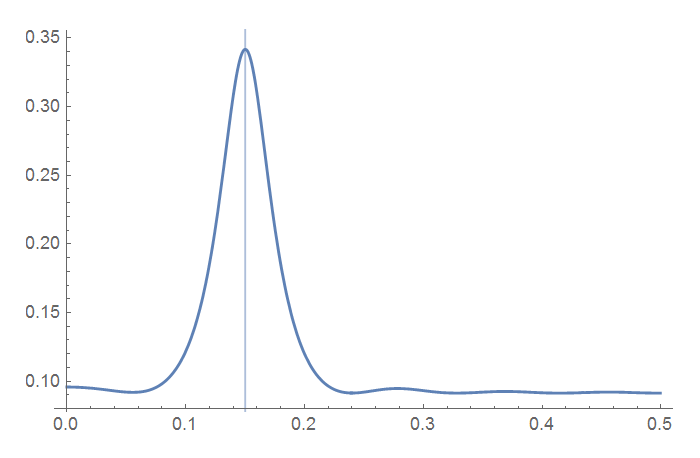
\includegraphics[width=0.8\textwidth]{pmd_f015_r1_p10}
        \caption{$\pmd\left(f\ge 0\right)$ синусоиды с шумом. Частота синусоиды $f_0=0.15$. Дисперсия шума $\rho=1$. Длина АКП $p=10$.}
        \label{fig:pmd_f015_r1_p10}
    \end{figure}

    Следовательно, по положению пиков горбов СПМ можно судить о частоте синусоиды, для которой эта СПМ была получена:
    \begin{equation}
        \hat{f_0} = \argmax\limits_{0 \le f \le {1 / {2 T}}} \pmd\left(f\right).
    \end{equation}
    $\hat{f_0}$ называется оценкой частоты.

    Можно показать, что оценка СПМ, а значит и частоты, по методу МД --- смещенная, причем смещение зависит от частоты $f_0$ синусоиды, длины $p$ АКП и дисперсии шума $\rho$: $\hat{f_0} = \hat{f_0}\left(f_0, p, \rho\right)$

    Смещение оценки, по определению, ${\mathrm B}\left(\hat{f_0}\right) = f_0 - \hat{f_0}$. В задаче предлагается исследовать смещение как функцию только длины $p$ АКП при фиксированных $f_0$ и $\rho$.

    На \autoref{fig:pmd_f015025045_r1} показана зависимость смещения оценки ${\mathrm B}\left(\hat{f_0}\right)={\mathrm B}\left[p\right]\left(\hat{f_0}\right)$ от $p$ для трех различных $f_0$. Можно заметить, что при фиксированной $f_0$ предел $\lim\limits_{p\to\infty}{\mathrm B}\left[p\right]={\mathrm B}\left[\infty\right] \ne 0$, что говорит о том, что оценка $\hat{f_0}$ --- смещенная.

    \begin{figure}
        \centering
        \captionsetup[subfigure]{labelformat=empty}
        \subfloat[$p=3$]{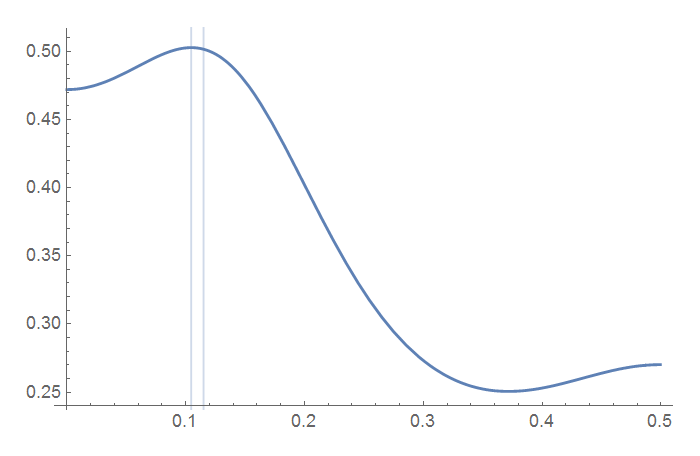
\includegraphics[height=1.5in]{pmd_f0115_r1_p3}}
        \subfloat[$p=4$]{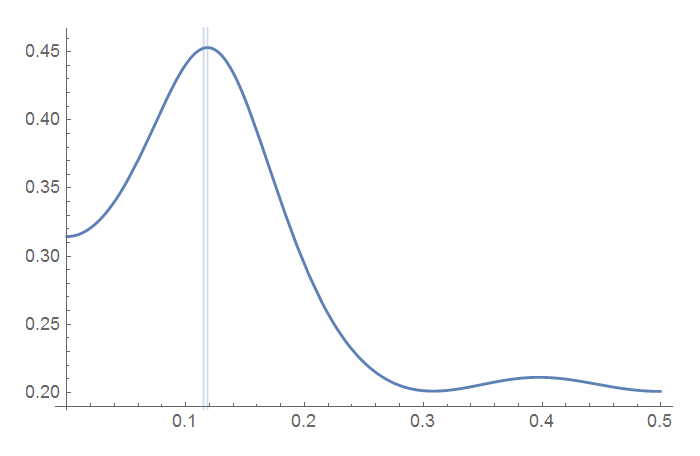
\includegraphics[height=1.5in]{pmd_f0115_r1_p4}}
        \subfloat[$p=5$]{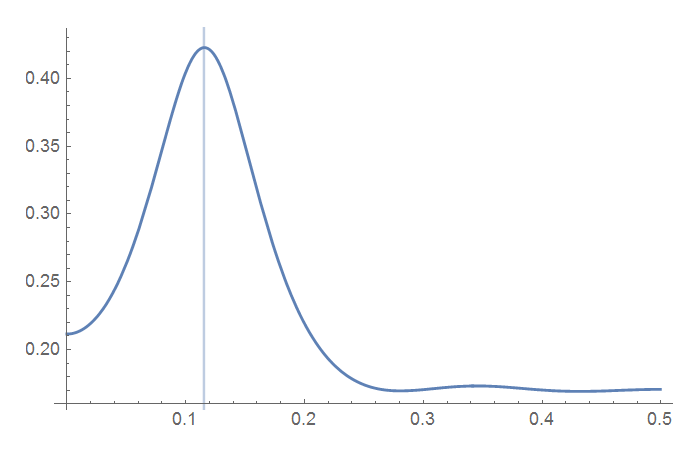
\includegraphics[height=1.5in]{pmd_f0115_r1_p5}}
        \caption{$\pmd\left(f\ge 0\right)$ синусоиды с шумом. Частота синусоиды $f_0=0.115$. Дисперсия шума $\rho=1$. Длина АКП --- $p$. Вертикальными линиями показаны $f_0$ и $\hat{f_0}$. Смещение оценки для $p=3,4$ видно невооруженным глазом. Видно также, что с ростом $p$ смещение уменьшается.}
        \label{fig:pmd_f0115_r1_p345}
    \end{figure}

    \begin{figure}
        \centering
        \captionsetup[subfigure]{labelformat=empty}
        \subfloat[$f_0=0.15$]{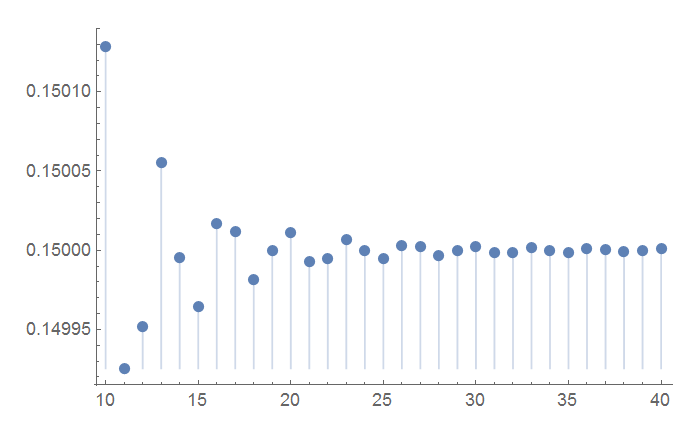
\includegraphics[height=1.5in]{pmd_f015_r1}}
        \subfloat[$f_0=0.25$]{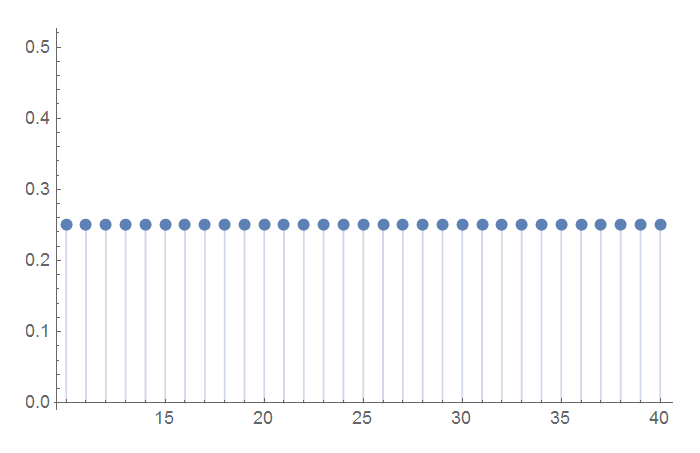
\includegraphics[height=1.5in]{pmd_f025_r1}}
        \subfloat[$f_0=0.45$]{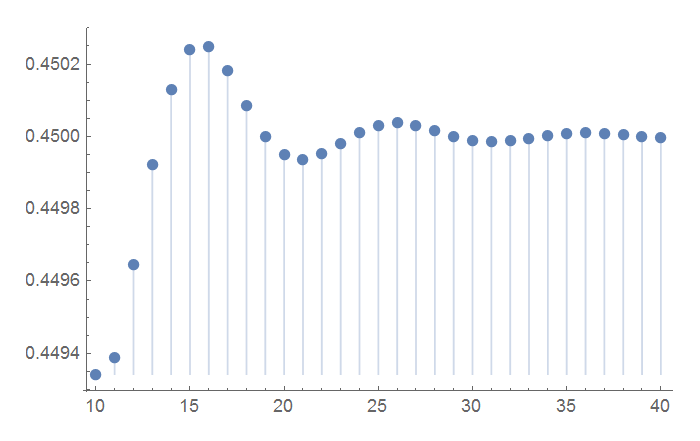
\includegraphics[height=1.5in]{pmd_f045_r1}}
        \caption{${\mathrm B}\left[p\right]$ синусоиды с шумом. Частота синусоиды --- $f_0$. Дисперсия шума $\rho=1$. Длина АКП $p=10 \div 40$. Видно, что с ростом $p$ смещение уменьшается. Видно также, что для разных частот $f_0$ смещения по-разному зависят от $p$, но все равно стремятся к некоторому (своему для каждой $f_0$) пределу ${\mathrm B}\left[\infty\right]$.}
        \label{fig:pmd_f015025045_r1}
    \end{figure}


    %% ===============================================
    %% =============== S1 ============================
    %% ===============================================

    \section{Реализация}

    \subsection{Общий алгоритм реализации}

    \begin{algorithm}
        \KwIn{$f_0,\;\rho,\;p_{min},\;p_{max}$}
        \KwOut{$\mathrm{B}\left[p\right]$}
        сформировать АКП $r\left[p\right]$, $p = p_{min} \div p_{max}$\;
        \For{$p = p_{min}$ \KwTo $p_{max}$}{
            получить $\pmd\left[p\right]$\;
            определить оценку $\hat{f_0}\left[p\right]$\;
            найти смещение оценки $\mathrm{B}\left[p\right]$\;
        }
        \caption{Получение смещения оценки от длины АКП \label{algo:general}}
    \end{algorithm}

    \subsection{Предлагаемая программная реализация}

    Предлагается следующая программная реализация задачи.

    \begin{listing}
        \caption{Максимально сжатый программный интерфейс задачи}
        \begin{cppcode}

            // глобальный максимум p, больше которого брать нельзя
            const int MAX_P_PLUS_ONE = 1000;

            // входные параметры
            double T, ro, f0;
            int    p_min, p_max /* < MAX_P_PLUS_ONE */;

            // выходные параметры
            double B[MAX_P_PLUS_ONE];

            // временные параметры
            double r[MAX_P_PLUS_ONE]; // АКП -> вычисление автокорреляционной матрицы
            double R_inv[MAX_P_PLUS_ONE][MAX_P_PLUS_ONE]; // обратная к автокорреляционной матрица -> вычисление one_to_sdp(f)

            // функции

            // m-й отсчет АКП
            double r_sin_with_noise(int m); // -> cos (2pi f0 T m) + ro delta (m)

            // обращение автокорреляционной матрицы
            void levinson_solve(int p); // -> заполняет R_inv[i][j], i,j = 0..p

            // вычисление знаменателя СПМ (т.е. 1 / СПМ) при частоте f
            // использует R_inv[i][j], i,j = 0..p
            double one_to_sdp(int p, double f);

            // ищет максимум СПМ (минимум 1 / СПМ)
            // возвращает координату пика СПМ
            // использует one_to_sdp как анализируемую функцию
            double find_max_sdp(int p);

            // считает смещение оценки для всех p = p_min..p_max
            // записывает данные в B[i], i=p_min..p_max.
            void bias();

            // главная функция

            // 1. ввод входных параметров
            // 2. вычисление r[i], i = 0..(MAX_P_PLUS_ONE-1)
            // 3. вызов bias
            // 4. вывод B[i], i = p_min..p_max
            void main();
        \end{cppcode}
    \end{listing}

    Приведенный код при должной его реализации решает поставленную задачу. Он составлен в полном соответствии с \autoref{algo:general}. Предлагается реализовать каждую функцию данного кода --- сначала в виде консольного приложения, а затем уже в виде графического приложения \begin{otherlanguage}{english}Windows\end{otherlanguage}. Также настоятельно рекомендуется реализовывать функции поэтапно --- сверху вниз --- с последующим тестированием. Следует обязательно сверить полученные результаты с рассчитанными, например, в \begin{otherlanguage}{english}Wolfram Mathematica\end{otherlanguage}. Особенно это касается решения СЛУ, поскольку алгоритм Левинсона, пожалуй, --- наиболее объемная часть программы.

    Функция \mintinline{c}{bias} может быть реализована следующим образом:

    \begin{listing}
        \caption{Псевдореализация функции \mintinline{c}{bias}}
        \begin{cppcode}
            void bias()
            {
                for (int p = p_min; p <= p_max)
                {
                    levinson_solve(p); // -> R_inv[i][j], i,j = 0..p
                    B[p] = f0 - find_max_sdp(p);
                }
            }
        \end{cppcode}
    \end{listing}

    В ней производится последовательное вычисление СПМ для различных $p$, поиск положения пика СПМ --- оценки $\hat{f_0} \equiv f_{estimated}$, вычисление смещения $\mathrm{B}\left[p\right]$.

    Стоит отметить, что функция \mintinline{c}{find_max_sdp} должна искать глобальный максимум. Так, если частота синусоиды достаточно близка к нулю, либо к $\pm 1 / {2 T}$, при малых $p$ метод минимума дисперсии может вовсе не разрешить частоту сигнала (\autoref{fig:pmd_f005_r1_p5}), а значит максимум СПМ будет находиться на границе области определения СПМ, соответственно, либо в $f = 0$, либо в $f = \pm 1 / {2 T}$. При реализации следует проверять на наличие максимума также и эти точки.

    \begin{figure}
        \centering
        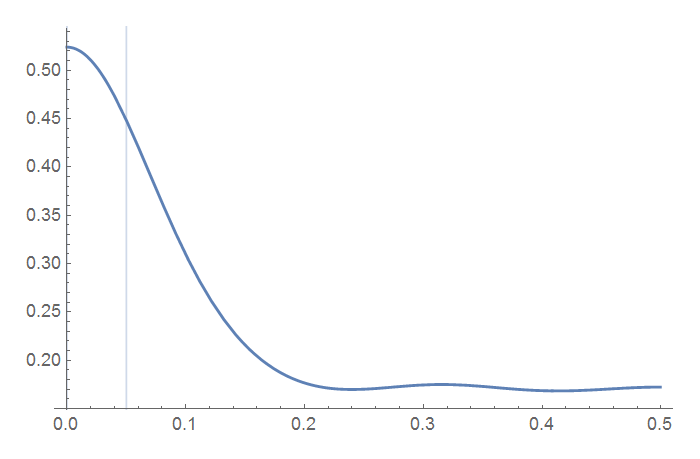
\includegraphics[width=0.8\textwidth]{pmd_f005_r1_p5}
        \caption{Пример неудовлетворительного разрешения метода МД. При частоте $f_0=0.05$ максимум СПМ достигается при $f=0$.}
        \label{fig:pmd_f005_r1_p5}
    \end{figure}

\end{document}

